%%%%%%%%%%%%%%%%%%%%%%%%%%%%%%%%%%%%%%%%%
% Masters/Doctoral Thesis
% LaTeX Template
% Version 2.5 (27/8/17)
%
% This template was downloaded from:
% http://www.LaTeXTemplates.com
%
% Version 2.x major modifications by:
% Vel (vel@latextemplates.com)
%
% This template is based on a template by:
% Steve Gunn (http://users.ecs.soton.ac.uk/srg/softwaretools/document/templates/)
% Sunil Patel (http://www.sunilpatel.co.uk/thesis-template/)
%
% Template license:
% CC BY-NC-SA 3.0 (http://creativecommons.org/licenses/by-nc-sa/3.0/)
%
%%%%%%%%%%%%%%%%%%%%%%%%%%%%%%%%%%%%%%%%%

%----------------------------------------------------------------------------------------
%	PACKAGES AND OTHER DOCUMENT CONFIGURATIONS
%----------------------------------------------------------------------------------------

\documentclass[
11pt, % The default document font size, options: 10pt, 11pt, 12pt
%oneside, % Two side (alternating margins) for binding by default, uncomment to switch to one side
english, % ngerman for German
singlespacing, % Single line spacing, alternatives: onehalfspacing or doublespacing
%draft, % Uncomment to enable draft mode (no pictures, no links, overfull hboxes indicated)
%nolistspacing, % If the document is onehalfspacing or doublespacing, uncomment this to set spacing in lists to single
%liststotoc, % Uncomment to add the list of figures/tables/etc to the table of contents
%toctotoc, % Uncomment to add the main table of contents to the table of contents
%parskip, % Uncomment to add space between paragraphs
%nohyperref, % Uncomment to not load the hyperref package
headsepline, % Uncomment to get a line under the header
%chapterinoneline, % Uncomment to place the chapter title next to the number on one line
%consistentlayout, % Uncomment to change the layout of the declaration, abstract and acknowledgements pages to match the default layout
]{MastersDoctoralThesis} % The class file specifying the document structure

\usepackage[utf8]{inputenc} % Required for inputting international characters
\usepackage[T1]{fontenc} % Output font encoding for international characters
\usepackage{float}
\usepackage{mathpazo} % Use the Palatino font by default

\usepackage[backend=bibtex,style=authoryear,natbib=true]{biblatex} % Use the bibtex backend with the authoryear citation style (which resembles APA)

\addbibresource{example.bib} % The filename of the bibliography

\usepackage[autostyle=true]{csquotes} % Required to generate language-dependent quotes in the bibliography

%----------------------------------------------------------------------------------------
%	MARGIN SETTINGS
%----------------------------------------------------------------------------------------

\geometry{
	paper=a4paper, % Change to letterpaper for US letter
	inner=2.5cm, % Inner margin
	outer=3.8cm, % Outer margin
	bindingoffset=.5cm, % Binding offset
	top=1.5cm, % Top margin
	bottom=1.5cm, % Bottom margin
	%showframe, % Uncomment to show how the type block is set on the page
}

%----------------------------------------------------------------------------------------
%	THESIS INFORMATION
%----------------------------------------------------------------------------------------

\thesistitle{DBMs Project: Online Public Access Catalogue} % Your thesis title, this is used in the title and abstract, print it elsewhere with \ttitle

\supervisor{Dr.Goliath \textsc{Li}} % Your supervisor's name, this is used in the title page, print it elsewhere with \supname
\examiner{} % Your examiner's name, this is not currently used anywhere in the template, print it elsewhere with \examname
\degree{Bachelor} % Your degree name, this is used in the title page and abstract, print it elsewhere with \degreename
\author{Junjie \textsc{LIU} \\ Yi \textsc{He}} % Your name, this is used in the title page and abstract, print it elsewhere with \authorname
\addresses{} % Your address, this is not currently used anywhere in the template, print it elsewhere with \addressname

\subject{Statistics} % Your subject area, this is not currently used anywhere in the template, print it elsewhere with \subjectname
\keywords{Statistics, DBMs} % Keywords for your thesis, this is not currently used anywhere in the template, print it elsewhere with \keywordnames
\university{\href{https://uic.edu.hk}{United International College}} % Your university's name and URL, this is used in the title page and abstract, print it elsewhere with \univname
\department{\href{http://dst.uic.edu.hk/}{Division of Science and Technology}} % Your department's name and URL, this is used in the title page and abstract, print it elsewhere with \deptname
%\group{\href{http://dst.uic.edu.hk/stat/}{Group S}} % Your research group's name and URL, this is used in the title page, print it elsewhere with \groupname
\faculty{\href{http://dst.uic.edu.hk/stat}{Statistics}} % Your faculty's name and URL, this is used in the title page and abstract, print it elsewhere with \facname

\AtBeginDocument{
\hypersetup{pdftitle=\ttitle} % Set the PDF's title to your title
\hypersetup{pdfauthor=\authorname} % Set the PDF's author to your name
\hypersetup{pdfkeywords=\keywordnames} % Set the PDF's keywords to your keywords
}

\begin{document}

\frontmatter % Use roman page numbering style (i, ii, iii, iv...) for the pre-content pages

\pagestyle{plain} % Default to the plain heading style until the thesis style is called for the body content

%----------------------------------------------------------------------------------------
%	TITLE PAGE
%----------------------------------------------------------------------------------------

\begin{titlepage}
\begin{center}

\vspace*{.06\textheight}
{\scshape\LARGE \univname\par}\vspace{1.5cm} % University name
\textsc{\Large Regression Analysis using R}\\[0.5cm] % Thesis type

\HRule \\[0.4cm] % Horizontal line
{\huge \bfseries \ttitle\par}\vspace{0.4cm} % Thesis title
\HRule \\[1.5cm] % Horizontal line

\begin{minipage}[t]{0.4\textwidth}
\begin{flushleft} \large
\emph{Author:}\\
{\authorname} % Author name - remove the \href bracket to remove the link
\end{flushleft}
\end{minipage}
\begin{minipage}[t]{0.4\textwidth}
\begin{flushright} \large
\emph{Supervisor:} \\
{\supname} % Supervisor name - remove the \href bracket to remove the link
\end{flushright}
\end{minipage}\\[3cm]

\vfill

%\large \textit{A thesis submitted in fulfillment of the requirements\\ for the degree of \degreename}\\[0.3cm] % University requirement text
%\textit{in the}\\[0.4cm]
\groupname\\\deptname\\\facname\\[2cm] % Research group name and department name


\vfill

{\large \today}\\[4cm] % Date
%\includegraphics{Logo} % University/department logo - uncomment to place it

\vfill
\end{center}
\end{titlepage}

%----------------------------------------------------------------------------------------
%	DECLARATION PAGE
%----------------------------------------------------------------------------------------

\begin{declaration}
\addchaptertocentry{\authorshipname} % Add the declaration to the table of contents
\noindent\authorname, declare that this thesis titled, \enquote{\ttitle} and the work presented in it are my own. I confirm that:

\begin{itemize}
\item This work was done wholly or mainly while in candidature for a research degree at this University.
\item Where any part of this thesis has previously been submitted for a degree or any other qualification at this University or any other institution, this has been clearly stated.
\item Where I have consulted the published work of others, this is always clearly attributed.
\item Where I have quoted from the work of others, the source is always given. With the exception of such quotations, this thesis is entirely my own work.
\item I have acknowledged all main sources of help.
\item Where the thesis is based on work done by myself jointly with others, I have made clear exactly what was done by others and what I have contributed myself.\\
\end{itemize}

\noindent Signed: Junjie \textsc{LIU} \ Yi \textsc{He}\\
\rule[0.5em]{25em}{0.5pt} % This prints a line for the signature

\noindent Date: \today \\
\rule[0.5em]{25em}{0.5pt} % This prints a line to write the date
\end{declaration}

\cleardoublepage


%----------------------------------------------------------------------------------------
%	ABSTRACT PAGE
%----------------------------------------------------------------------------------------

\begin{abstract}
\addchaptertocentry{\abstractname} % Add the abstract to the table of contents
Lots of institutions or individuals have begun to set up private libraries. Book management has also become an indispensable part of daily management and the core of everyday things in the library. In the past, people used paper documents to record the borrowing of books. This method of recording is not only cumbersome but also error-prone. With the development of IT technology in recent years, it has become possible to develop a simple and practical library management system. Previously, there were development systems in various languages, but the pertinence was not strong. Now, develop a simple, practical library management system for small or medium-sized books to meet the needs.
\end{abstract}

%----------------------------------------------------------------------------------------
%	ACKNOWLEDGEMENTS
%----------------------------------------------------------------------------------------

%\begin{acknowledgements}
%\addchaptertocentry{\acknowledgementname} % Add the acknowledgements to the table of contents
%We would like to dedicate this dissertation to our teachers, Dr.Ye Hua Jun, Dr.He Ping, also, our Teacher Asistant Jenna, without their helps, we would not able finish this report. Also, Thanks to the Statistics Labtoray, which provides the computers\dots
%\end{acknowledgements}

%----------------------------------------------------------------------------------------
%	LIST OF CONTENTS/FIGURES/TABLES PAGES
%----------------------------------------------------------------------------------------

\tableofcontents % Prints the main table of contents

\listoffigures % Prints the list of figures

%\listoftables % Prints the list of tables

%----------------------------------------------------------------------------------------
%	ABBREVIATIONS
%----------------------------------------------------------------------------------------

%\begin{abbreviations}{ll} % Include a list of abbreviations (a table of two columns)

%\textbf{OLR} & \textbf{O}rdinary \textbf{A}bbreviations \textbf{H}ere\\
%\textbf{WSF} & \textbf{W}hat (it) \textbf{S}tands \textbf{F}or\\

%\end{abbreviations}

%----------------------------------------------------------------------------------------
%	PHYSICAL CONSTANTS/OTHER DEFINITIONS
%----------------------------------------------------------------------------------------

%\begin{constants}{lr@{${}={}$}l} % The list of physical constants is a three column table

% The \SI{}{} command is provided by the siunitx package, see its documentation for instructions on how to use it

%Speed of Light & $c_{0}$ & \SI{2.99792458e8}{\meter\per\second} (exact)\\
%Constant Name & $Symbol$ & $Constant Value$ with units\\

%\end{constants}

%----------------------------------------------------------------------------------------
%	SYMBOLS
%----------------------------------------------------------------------------------------

%\begin{symbols}{lll} % Include a list of Symbols (a three column table)

%%$a$ & distance & \si{\meter} \\
%$P$ & power & \si{\watt} (\si{\joule\per\second}) \\
%Symbol & Name & Unit \\

%\addlinespace % Gap to separate the Roman symbols from the Greek

%$\omega$ & angular frequency & \si{\radian} \\

%\end{symbols}

%----------------------------------------------------------------------------------------
%	DEDICATION
%----------------------------------------------------------------------------------------

%\dedicatory{For/Dedicated to/To my\ldots}

%----------------------------------------------------------------------------------------
%	THESIS CONTENT - CHAPTERS
%----------------------------------------------------------------------------------------

\mainmatter % Begin numeric (1,2,3...) page numbering

\pagestyle{thesis} % Return the page headers back to the "thesis" style

% Include the chapters of the thesis as separate files from the Chapters folder
% Uncomment the lines as you write the chapters

% Chapter 1

\chapter{Introduction} % Main chapter title

\label{Chapter1} % For referencing the chapter elsewhere, use \ref{Chapter1}

%----------------------------------------------------------------------------------------

% Define some commands to keep the formatting separated from the content
\newcommand{\keyword}[1]{\textbf{#1}}
\newcommand{\tabhead}[1]{\textbf{#1}}
\newcommand{\code}[1]{\texttt{#1}}
\newcommand{\file}[1]{\texttt{\bfseries#1}}
\newcommand{\option}[1]{\texttt{\itshape#1}}

%********************************** %First Section  **************************************
\section{Background} %Section - 1.1

This article describes the design of a small or medium-sized library management system. Focusing on the technical perspective, the planning of the small and medium-sized library database management system and the design of the main function modules are discussed.
The libraries described in this article are not the same as the public library, but also different from the higher school library. The main manifestations are:
(1) From the perspective of the book star, it belongs to the small and medium-sized (generally in the tens of thousands of volumes). Due to the limited funds, the distribution of the types of books is closely related to the professional settings of the institutions.
(2) The number of readers is limited (generally around a thousand people), and the time rules for book retrieval and borrowing are strong. ( ) 3 There are fewer library staff, which makes the professional division of labor less clear, and often one person has several positions.
In order to improve the quality of the book collection, use the limited collection of books more effectively, provide readers with high-quality services, and make the management of the library scientific and modern, we have developed a library database system on the microcomputer, system development. Fully consider the characteristics of the secondary professional school library, and strive to make it have the management functions of small and medium-sized libraries.
This Library management system requires the ability to divide and set the features and permissions of books, readers, system administrators and other roles. The system is required to operate correctly and the operation interface is simple and easy to understand.


%********************************** %Second Section  *************************************
\section{System's Objective} %Section - 1.2

The main functions of the system are: it can manage the system user information and permissions, can manage the book information, can manage the reader information, can carry out the book borrowing operation and record the borrowing information. After the group discussion, the system should mainly have the following Features:

\begin{itemize}
    \item \textbf{Features One:} Modify book information, manage system administrators and set up all departments, manage bookshelf number and save books, exit system;
    \item \textbf{Features Two:} Manage reader information and types, new users can register themselves, administrators have the permission to add or delete users;
    \item \textbf{Features Three:} Borrow books, return books, check loan's status;
    \item \textbf{Featrues Four:} Add "Groups", to let readers with similar interests discuss in the same group; administrators can create new groups, users can join groups
\end{itemize}

\section{Introduction to system flow}

\begin{figure}[htbp!]
\centering
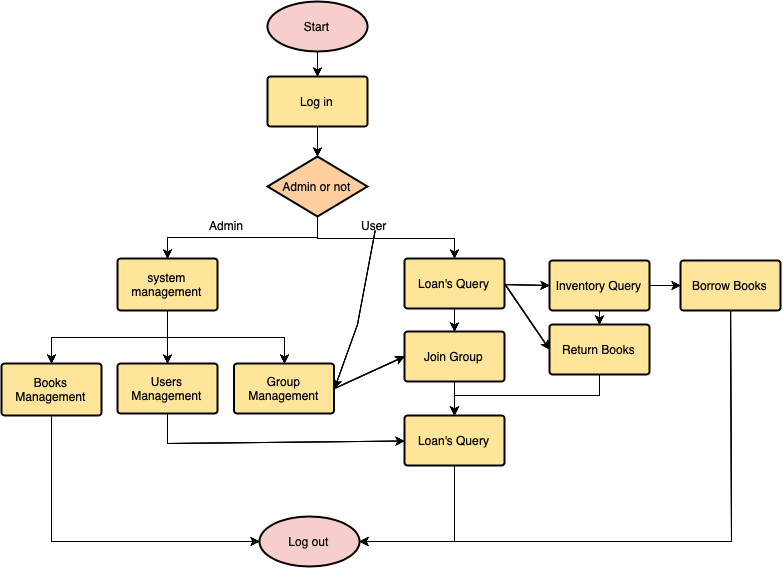
\includegraphics[width=1.0\textwidth]{Figures/Flowchart.png}
\caption[Figures/origindata.png]{Flowchart}
\label{fig:System Flow Chart}
\end{figure}

% Chapter Template

\chapter{System Implement} % Main chapter title

\label{Chapter2} % Change X to a consecutive number; for referencing this chapter elsewhere, use \ref{ChapterX}

\section{System Structure}

According to the actual needs of the library management system, the library management system can be divided into system management, reader management, library management, borrowing management, query, book ranking, and the specific functions of the various parts of the system module architecture diagram shown in \fig{Origni data Set} .

\begin{figure}[htbp!]
\centering
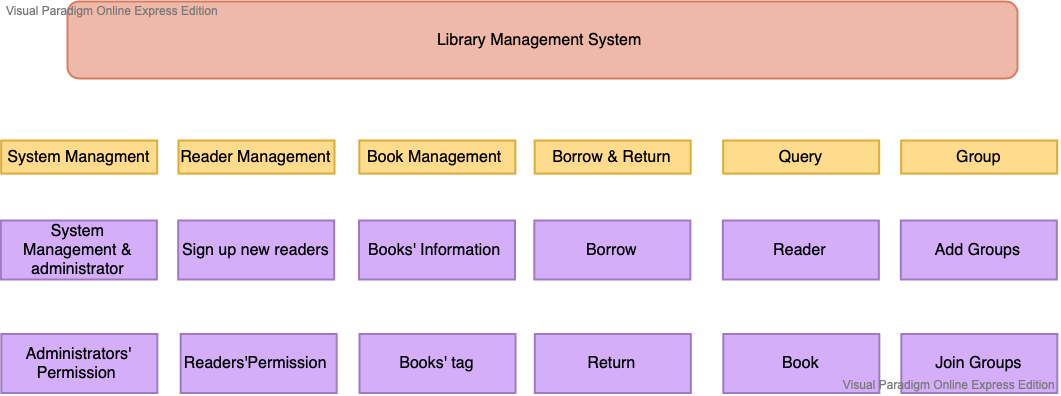
\includegraphics[width=1.0\textwidth]{Figures/structure.png}
\caption[Figures/origindata.png]{System Structure}
\label{fig:System Structure}
\end{figure}


The data set we chosen is from the UCI Machine Learning Repository datasets, it has collected Beijing PM2.5 data from 2010 to 2014. In this data sets, its collection is based on hours, and from the original data set we can see that there are lots of missing value (approximately $4.7\%$ data of PM2.5 are missing). We need to delete the missing data. In order to reduce the impact of deleting missing values on data, we select the data of the fourth year and fifth year, namely 2013 and 2014 respectively.


\section{Time Data Processing}
As we have mentioned before, the PM2.5 maybe have a high co-linearity with time (a few hours a day, a few days a month, a few months a year), and in the time-series data, there usually auto-correlation between the  in order to ignore this time series problem, we decided to reduce this correlation through some data processing procedures.

After setting up the full model, we discover that the R square is insignificant, then we separate the data into two classes: Summer and Autumn, Spring and Winter. We do the model estimation. Then, we classified them again and now the data are in four classes. In order to select the most appropriate categorical variable, we believe that the PM2.5 level is related to the weather. For weather data, it is usually seasonal. For example, we expect winter air pollution to become more severe as coal consumption increases. Therefore, we decided to change only the classification predictor for the seasons to categorical variables.

At the same time, the wind direction and wind force will also affect the concentration of PM2.5 every day. Since the original data set has no wind data, only the hourly wind direction, and the current data set needs the average wind direction of each day, and the average wind direction calculation. It is divided into two methods, the averaging method and the vector summation method \citep{yueh1997modeling}. In order to eliminate the "wind strength" required in the "vector summation method", we choose to use the averaging method for calculation.

In addition, through the lubridate package in the R language, we convert the character variable "time" into a numeric variable: timestamp.

In the end, the new data set contains eight independent variables and one dependent variables:

\begin{figure}[h!]
\centering
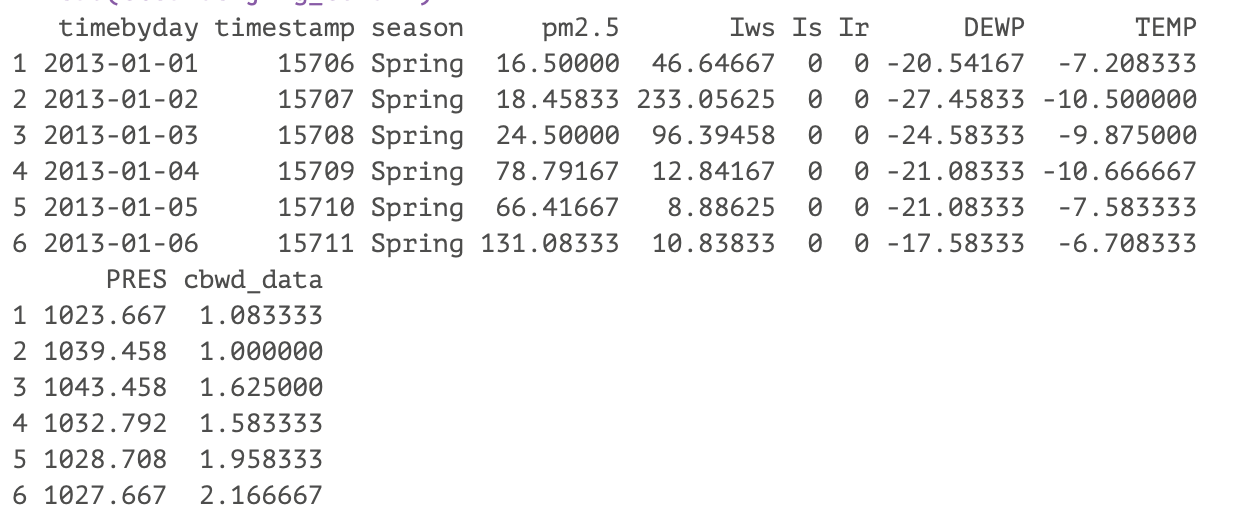
\includegraphics[width=1.0\textwidth]{Figures/newdata.png}
\caption[Figures/newdata.png]{new data set}
\label{fig:new data set}
\end{figure}

% Chapter Template
\chapter{Original Data Analysis} % Main chapter title

\label{Chapter3} % Change X to a consecutive number; for referencing this chapter elsewhere, use \ref{ChapterX}

%----------------------------------------------------------------------------------------
%	SECTION 1
%----------------------------------------------------------------------------------------

\section{Full Model Estimation}

 As we have mentioned, we did the data pre-processing before we begin our data analysis (model fitting). We analyzed this set of data according to the most
 fundamental steps of regression analysis. This is the analysis of the full model.
Our Full model's regression formula is :

\begin{align*}
  \centering
PM2.5 = \beta_0 + \beta_1\text{timestamp} + \beta_2\text{season} + \beta_3\text{Iws} + \beta_4\text{Is} + \beta_5\text{Ir} + \beta_6\beta\text{DEWP} + \beta_7\text{TEMP} + \beta_8\text{PRESS} + \beta_9\text{cbwd_data}
\end{align*}


The model's summary are given below:
\\
\\
\begin{tabular}{|c|c|c|c|c|}
\hline       beta   &    Estimate & Std. Error &t value &Pr(>|t|)    \\
\hline (Intercept)  & 2.344e+03  &5.414e+02 &  4.329 &1.71e-05 *** \\
\hline timestamp    & -4.383e-04 & 1.178e-02&  -0.037& 0.970337    \\
\hline seasonSpring & 2.530e+01  &8.012e+00  & 3.158 &0.001654 **  \\
\hline easonSummer  & -3.362e+01 & 8.985e+00 &-3.742 &0.000197 *** \\
\hline seasonWinter & 2.408e+01  &9.346e+00  & 2.576 &0.010193 *   \\
\hline Iws          & -1.657e-01 & 6.586e-02 & -2.516& 0.012075 *   \\
\hline Is           & -1.544e+01 & 6.509e+00 & -2.372& 0.017953 *   \\
\hline Ir           & -1.493e+01 & 2.967e+00 & -5.032 &6.13e-07 *** \\
\hline DEWP         & 7.567e+00  &5.021e-01  &15.070  &< 2e-16 *** \\
\hline TEMP         & -1.053e+01 & 7.359e-01 &-14.310 & < 2e-16 *** \\
\hline PRES         & -2.056e+00 & 5.292e-01 & -3.885 &0.000112 *** \\
\hline cbwd\_dataNE  & -6.115e+01 & 1.226e+01 & -4.988 &7.66e-07 *** \\
\hline cbwd\_dataNW  & -2.927e+01 & 7.431e+00 & -3.939 &9.00e-05 *** \\
\hline cbwd\_dataSE  & -1.883e+01 & 6.793e+00 & -2.772 &0.005710 **  \\
\hline
\end{tabular}
\\
\\

Which is in the form of: $y = \beta_1 x_1 + \dots + \beta_9 x_9 \label{eq: Full Model}$

Initally, to come up with the full model, we decided to first plot correlation plots for all regressors that we believed taht may have a constant variance: See \refeq{fig:Correlation of the full model}

\begin{figure}[H]
    \centering
  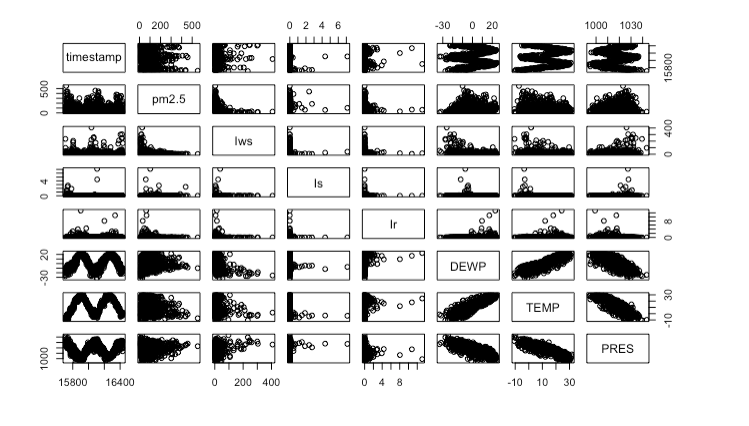
\includegraphics[width=1.0\textwidth]{Figures/correlationfull.png}
  \caption[Figures/correlation\_full.png]{Correlation of the full model}
  \label{fig:Correlation of the full model}
\end{figure}

From \ref{fig:Correlation of the full model}, we noticed that the correlation between PM2.5 and cumulated hour of wind speed(Iws), cumulative hours of snow(Is), and cumulative hours of rain(Ir) are all strong and their correlation density curve  seem like all right skewed. We can use the 'Residuals vs Fitted' plot and the 'Normal Q-Q' plot of residual to check whether our deduction.


The $`lm`$ function can also plots out the 'Residuals vs Fitted' plot, 'Normal Q-Q'plot, 'Scale-Location' and 'Residuals vs Leverage' plot: See \refeq{fig:Testing Plots of Full Model}

\begin{figure}[H]
  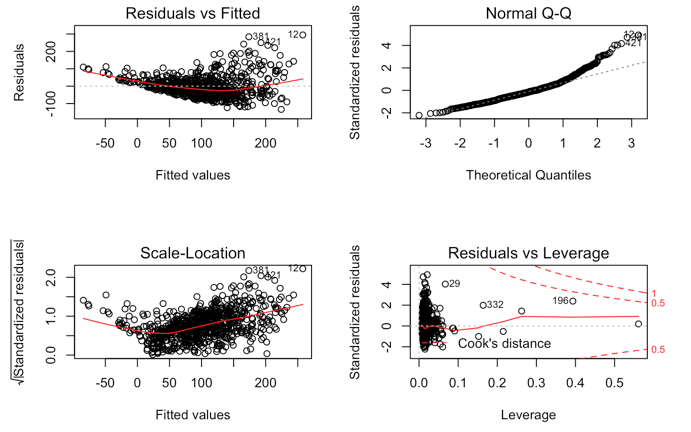
\includegraphics[width=1.0\textwidth]{Figures/lm_full.png}
  \caption[Figures/lm\_full.png]{Four testing plots}
  \label{fig:Testing Plots of Full Model}
\end{figure}

We also use lm and vif function to check the vif value of each variables. The result shows that all the variables’ vif value are not way larger than 10. The largest one is approximately $13.4$, which means the variables don’t have a high multicolliearity and the model has no compressibility. We can’t do the ridge regression and also the lasso regression to this model.

\section{Model with Natural Logrithm}
It can be seen that the residual of the  full model \ref{eq: Full Model} is nonlinear. Usually, we need to do the \textbf{ncv test} to check want kinds of transformation should we do, however, according the reference book, we can do the Natural Logarithm transforamtion to the dependent variable when the residual plot is right skewed the\citep{montgomery2012introduction}.  Then we take the natural logarithm of the dependent variable, thus obtaining a new regression model: Full Model with Natural Logarithm Transformation, by comparing the residual graphs of the two models, we can clearly see that the residual of the model after natural logarithm transformation is linear, but we can see the residuals plot as the double-bow model\citep{montgomery2012introduction}, which represents the model at this time. The variance of the residuals is not the same, and it does not satisfy the characteristics of the regression model of homoscedasticity.

Here is the formula of the model after the Natural Logarithm transformation:

\begin{align*}
  \centering
  log(PM2.5) = \beta_0 + \beta_1\text{timestamp} + \beta_2\text{season} + \beta_3\text{Iws} + \beta_4\text{Is} + \beta_5\text{Ir} + \beta_6\beta\text{DEWP} + \beta_7\text{TEMP} + \beta_8\text{PRESS} + \beta_9\text{cbwd_data}
\end{align*}
Which is in form of :
$log(y) = \beta_1 x_1 + \dots + \beta_9 x_9 \label{eq: Full Model with Natural Logarithm}$

\begin{figure}[H]
  \centering
  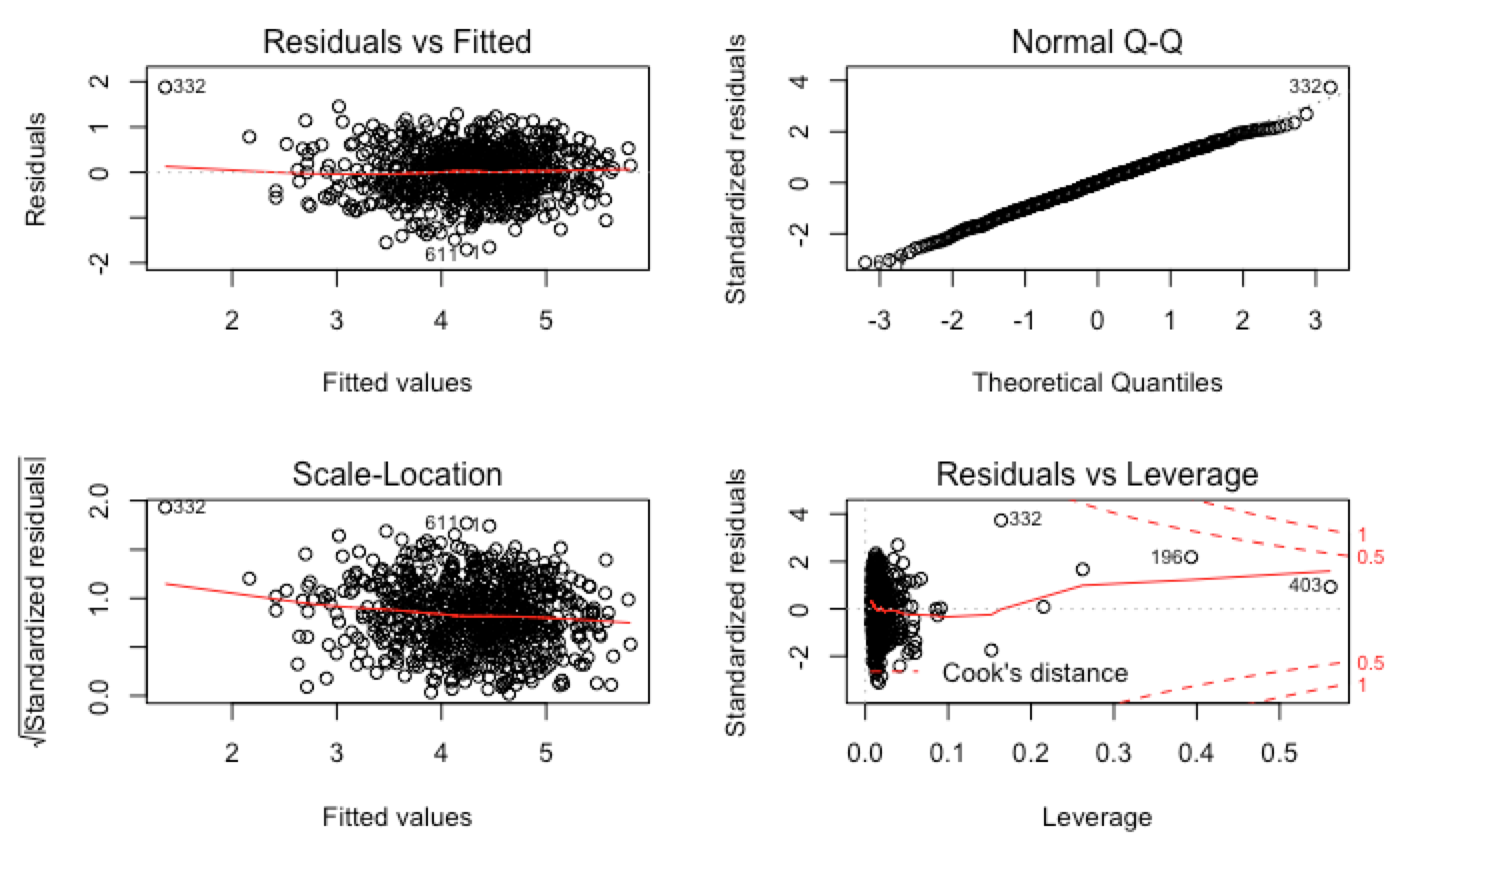
\includegraphics[width=1.0\textwidth]{Figures/lm_full_nl.png}
  \caption[Figures/lm\_full\_nl.png]{Full Model with Natural Logarithm test plot}
  \label{fig:Full Model with Natural Logarithm test plot}
\end{figure}

\section{Interaction Model}
According to the \ref{fig:Correlation of the full model}, there are some correlations between some of the independent variables and dependent variable,
It can be seen that although the residual at this time is in accordance with the normal distribution, it can be seen from the residual map that the variance of the residuals is not the same. We suspect that there are interactions between different variables, so we have newly created a model to try to improve the $R^2$ of the model, and then filter the model through stepwise method.

The Interaction Model is:
\\
\\
\begin{align*}
  \centering
  log(PM2.5) = ()\beta_0 + \beta_1\text{timestamp} + \beta_2\text{season} + \beta_3\text{Iws} + \beta_4\text{Is} + \beta_5\text{Ir} + \beta_6\beta\text{DEWP} + \beta_7\text{TEMP} + \beta_8\text{PRESS} + \beta_9\text{cbwd_data})^2
\end{align*}
\\
\\
\begin{figure}[H]
  \centering
  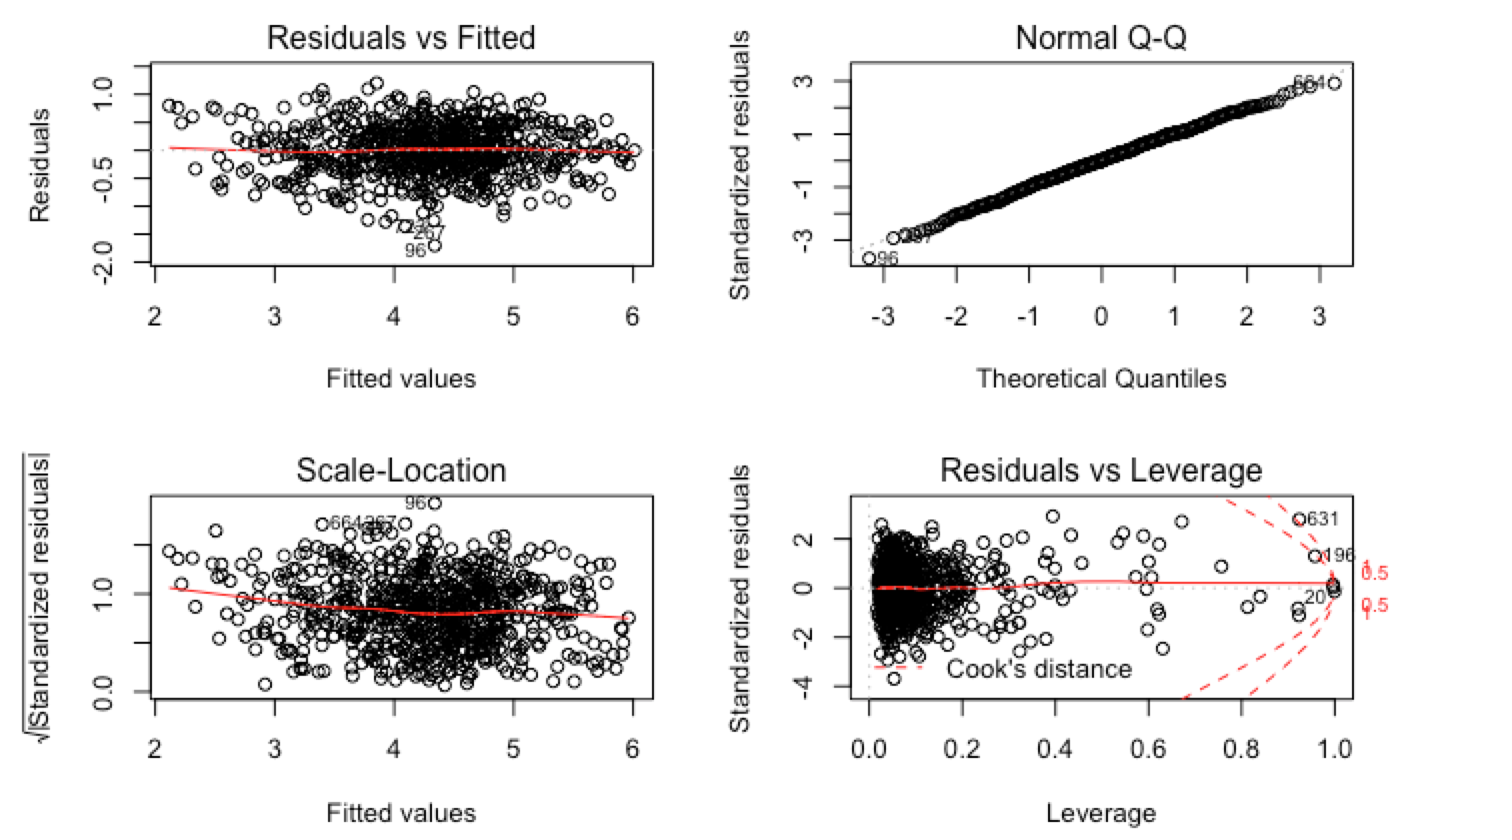
\includegraphics[width=1.0\textwidth]{Figures/lm_full_in.png}
  \caption[Figures/lm\_full\_in.png]{Natural Logarithm Model with Interaction}
  \label{fig:Natural Logarithm Model with Interaction}
\end{figure}

As we can see in the \ref{fig:Natural Logarithm Model with Interaction}, the  variance is more dispersed, the homoscedasticity is better, and R square($R^2 = 0.7086$) is higher.

\section{Stepwise Method}

In Statistics, we usually use Stepwise to choose the variables, choose the predictive varaibles by the R's built-in automatic procedure.
At the beginning, the AIC = $-1001.82$ and at the last step, the AIC = $-1035,45$, and the
model selected by AIC is:

\begin{align*}
\centering
log(pm2.5)  = timestamp + season + Iws + Is + Ir + DEWP + TEMP +
    PRES + cbwd_data + timestamp:season + timestamp:Is + timestamp:cbwd_data +
    season:Iws + season:DEWP + season:TEMP + season:PRES + season:cbwd_data +
    Iws:Ir + Iws:DEWP + Iws:TEMP + Iws:PRES + Iws:cbwd_data +
    Is:TEMP + Is:PRES + Ir:DEWP + Ir:TEMP + Ir:PRES + DEWP:PRES +
    TEMP:cbwd_data + PRES:cbwd_data + intercept
\end{align*}
The R square now is $0.6995$ and the test plots is much better than before, see \ref{fig:Stepwise Model}
\begin{figure}[H]
  \centering
  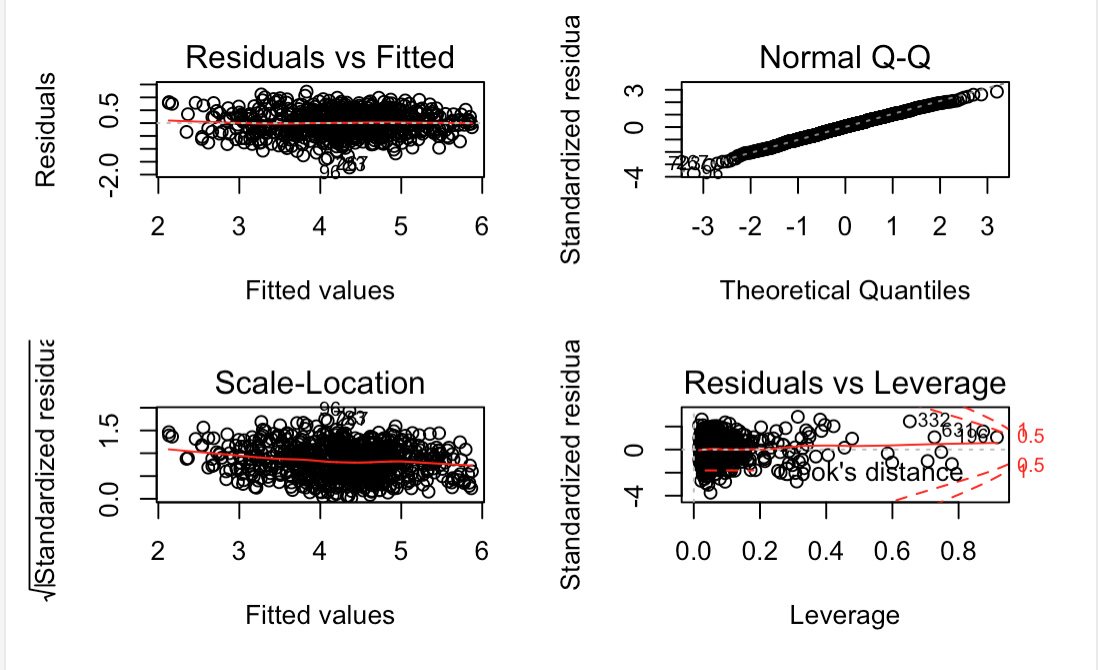
\includegraphics[width=1.0\textwidth]{Figures/lm_full_in_step.png}
  \caption[Figures/lm\_full\_in\_step.png]{Stepwise Model}
  \label{fig:Stepwise Model}
\end{figure}
Although it seem like a good model, in some ways, we thought it was not a fitted model we want.
After checking the original variables again, we found that the Cumulated hours of snow , Dew Point and Temperature thereT all have strong correlation with time. Then, we came up a new idea, we have to separate the time as a more smaller segments in terms of season as unit. Usually, smog is more likely to affect humans in the spring and winter seasons. This can be reflected in the previous model. The correlation between spring and winter and pm2.5 is much larger than that in summer and autumn.
Then, we chose Spring + Winter as the time nodes and continue our model estimation.

% Chapter Template

\chapter{New Model Esitmation and Data Diagnostics} % Main chapter title

\label{Chapter 4} % Change X to a consecutive number; for referencing this chapter elsewhere, use \ref{ChapterX}
\section{Spring Winter Model}
By using the `lm` function from the car package, we find that spring and winter are significant than two other seasons. See:  \refeq{fig:Coefficient Plot}

\begin{figure}[H]
  \centering
  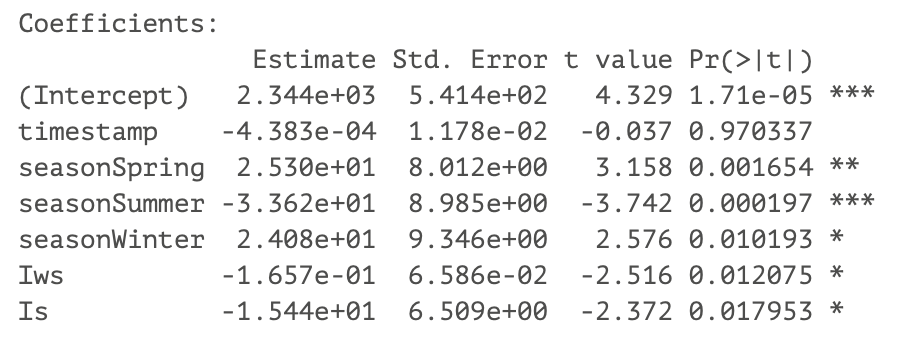
\includegraphics[width = 1.0\textwidth]{Figures/coef_full.png}
  \caption[Figures/coef\_full.png]{Coefficient Plot}
  \label{fig:Coefficient Plot}
\end{figure}

So, we decide to grouping the data into two parts. Spring-Winter data as one set and the Summer-Autumn data as another set. Then we use the lm function to compare these two models and find that the Spring-Winter Model is better than the other one.

\begin{figure}[H]
  \centering
  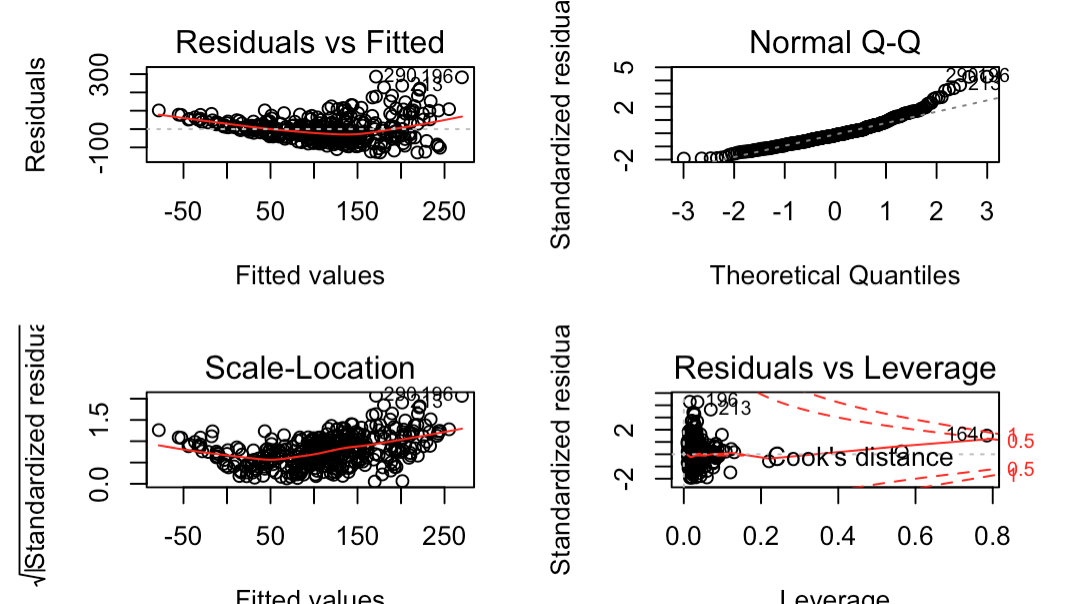
\includegraphics[width = 1.0\textwidth]{Figures/spring_winter.png}
  \caption[Figures/spring\_winter.png]{Spring Winter Model}
  \label{fig:Spring_Winter Model}
\end{figure}


From the plots we can see that there is not linear correlation between these variables. We thus do the ncvTest and draw the spreadlevel plot, the suggested power transformation is 0.381492.\citeq{Kabacoff2015} See: \refeq{fig:NCVTest}

\begin{figure}[H]
  \centering
  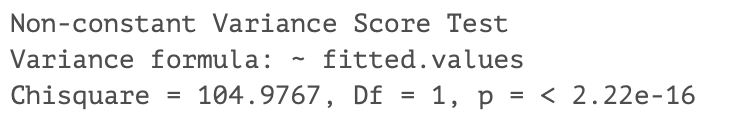
\includegraphics[width = 1.0\textwidth]{Figures/ncv.png}
  \caption[Figures/ncv.png]{NCV Test}
  \label{fig:NCVTest}
\end{figure}

\begin{figure}[H]
  \centering
  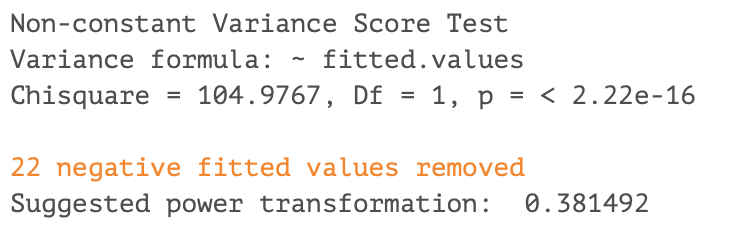
\includegraphics[width = 1.0\textwidth]{Figures/ncv_spread.png}
  \caption[Figures/ncv_spread.png]{NCV Test and Suggested Power Transformation}
  \label{fig:NCV Test and Suggested Power Transformation}
\end{figure}

\begin{figure}[H]
  \centering
  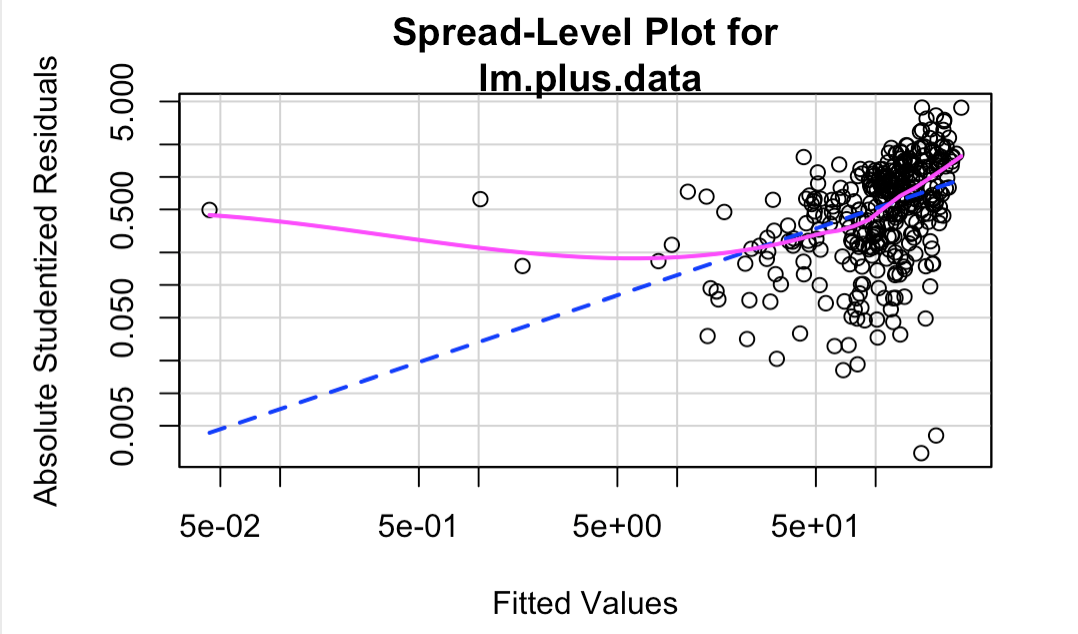
\includegraphics[width = 1.0\textwidth]{Figures/spread.png}
  \caption[Figures/spread.png]{Spreadlevel Plot}
  \label{fig:Spreadlevel Plot}
\end{figure}

. We think it may means closed to $0.5$ or closed to $0$. First, we take square loot to the pm2.5, but the result ignores our consideration. Then we start to consider another possibility, which is closed to $0$, meaning we should take the natural logarithm to the pm2.5. We wonder what will happen if we take the natural logarithm to the pm2.5. We use lm function again to estimate the Spring-Winter Model with natural logarithm and the results shows the linear correlation. Also, the residual plots and the R square are both better than before.

\begin{figure}[H]
  \centering
  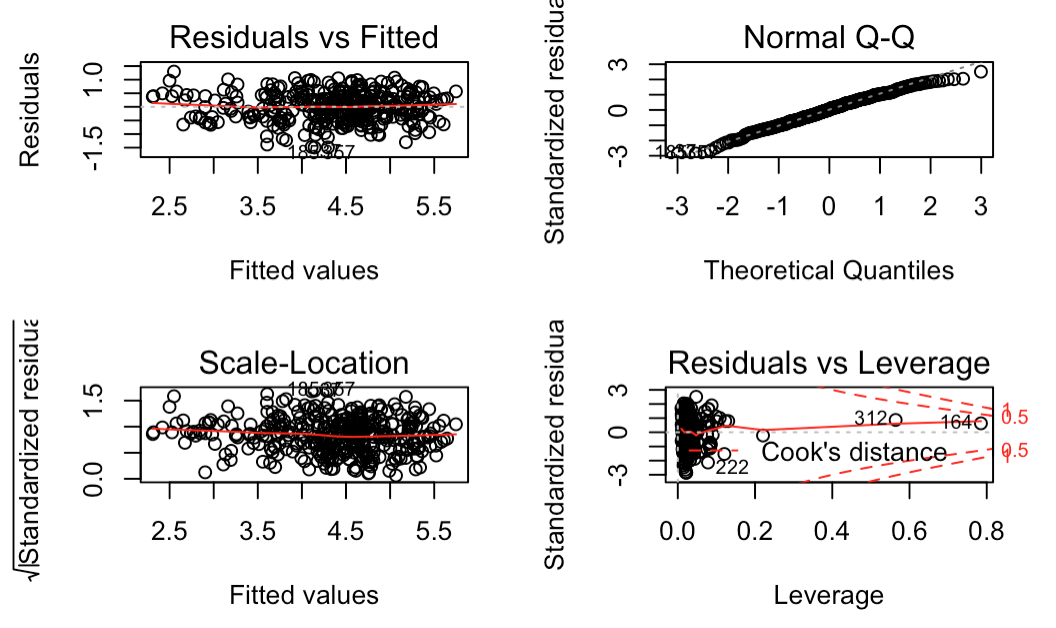
\includegraphics[width = 1.0\textwidth]{Figures/spring_winter_nl.png}
  \caption[Figures/spring\_winter\_nl.png]{Natural Logarithm of Spring Winter Model}
  \label{fig:Natural Logarithm of Spring Winter Model}
\end{figure}

From the full model vif figure, the vif value of the winter is the most significant one in four single seasons. With this discovery, we choose the winter data to form a model with natural logarithm. Also, we form a model for the spring data with natural logarithm, but it is not good as the winter one.

\begin{figure}[H]
  \centering
  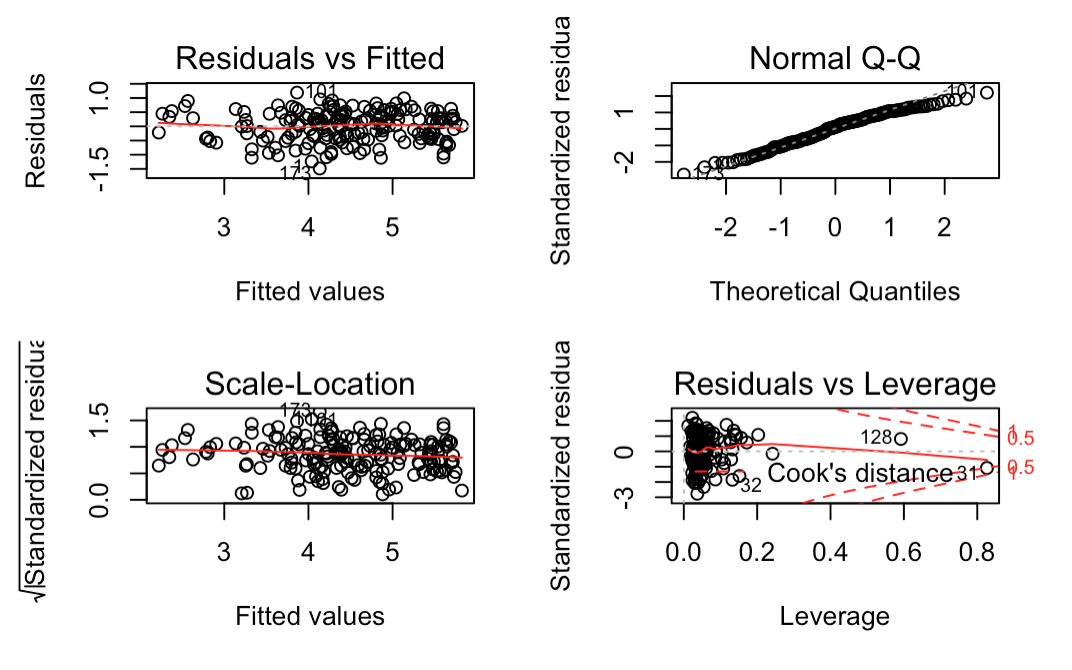
\includegraphics[width = 1.0\textwidth]{Figures/winter_nl.png}
  \caption[Figures/winter\_nl.png]{ Winter Model Natural Logarithm}
  \label{fig: Winter Model Natural Logarithm}
\end{figure}

The Formula of Winter Model with Natural Logarithm is :

\begin{align*}
  log(pm2.5)  = \beta_1 timestamp + \beta_2 Iws + \beta_3 Is + \beta_4 Ir + \beta_5 DEWP +
    \beta_6 TEMP + \beta_7 PRES + \beta_8 cbwd_data \label{eq: Winter Model with Natural Logarithm}
\end{align*}

 The residual plots are better and the R square is higher than what we have found out before.
So we use this model \ref{eq: Winter Model with Natural Logarithm} to do the regression model diagnostics.

\begin{figure}[H]
  \centering
  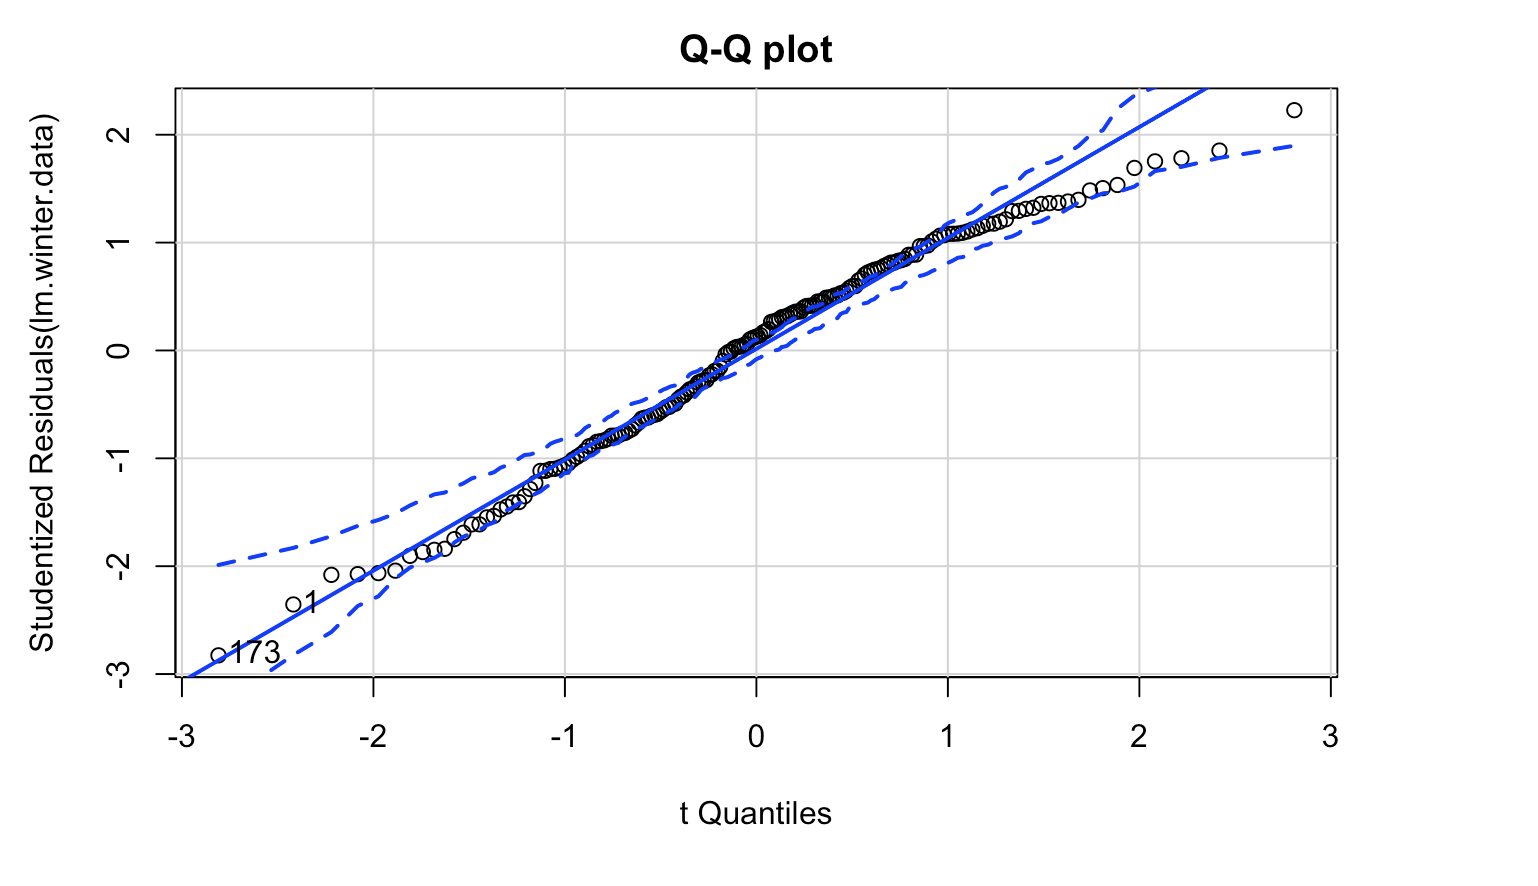
\includegraphics[width = 1.0\textwidth]{Figures/QQ.png}
  \caption[Figures/QQ.png]{Q-Q Plot}
  \label{fig: Q-Q Plot}
\end{figure}

First, we draw the Q-Q plot, the plot shows that all the points are closed to the straight line, and they are all in the confident interval, which means the normality assumption of this Winter Natural Logarithm Model is good.
We also use the residplot function to draw the Studentized Residual Histogram, and add the Normal Curve, Kernel Density Curve and Rug Plot.

\begin{figure}[H]
  \centering
  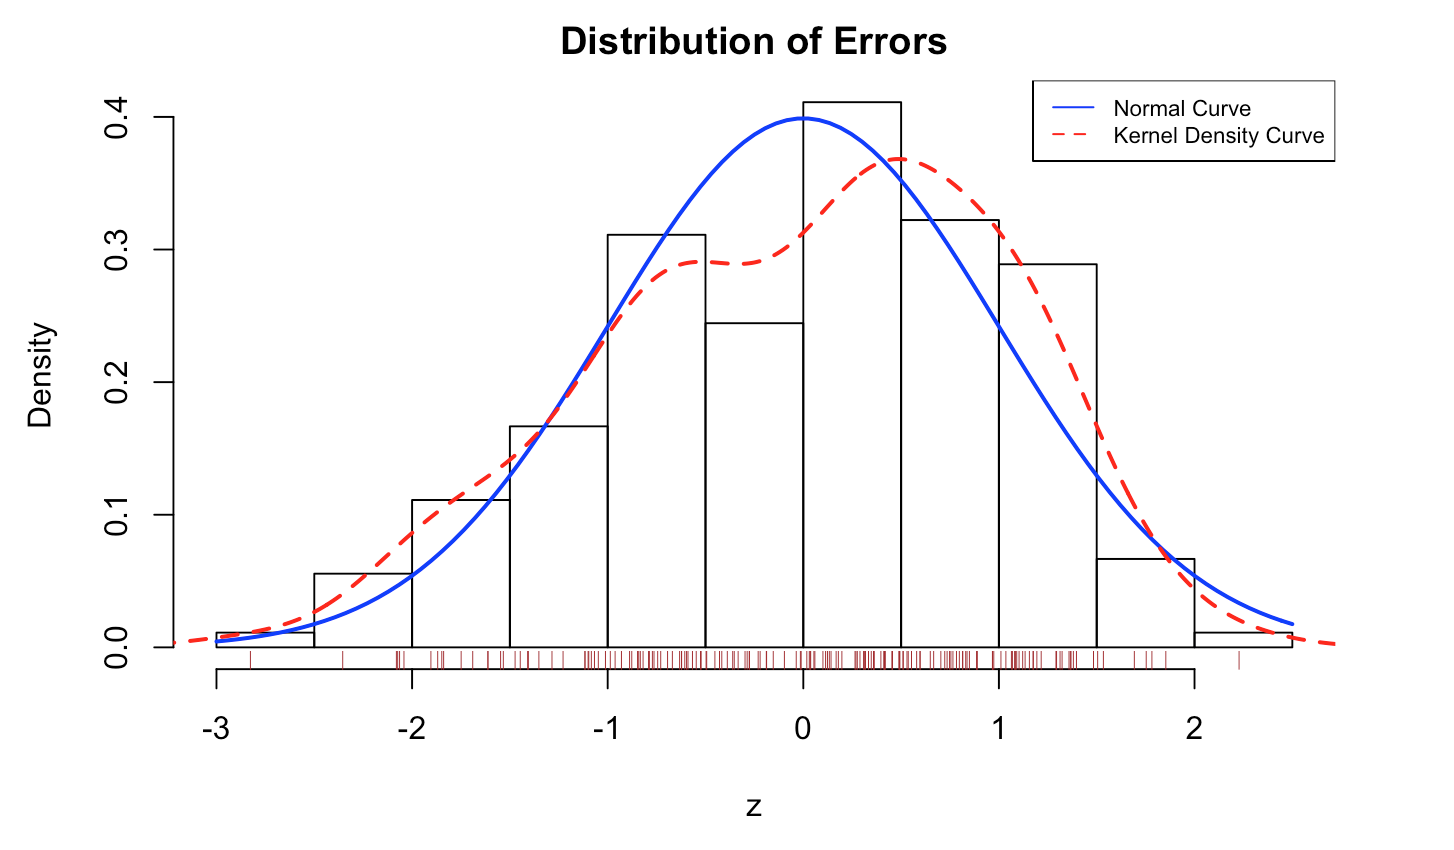
\includegraphics[width = 1.0\textwidth]{Figures/density.png}
  \caption[Figures/density.png]{Studentized Residual Density Plot}
  \label{fig: Studentized Residual Density Plot}
\end{figure}

% Chapter Template

\chapter{Conclusion} % Main chapter title

\label{Chapter5} % Change X to a consecutive number; for referencing this chapter elsewhere, use \ref{ChapterX}

%----------------------------------------------------------------------------------------
%	SECTION 1
%----------------------------------------------------------------------------------------
\section{Conlcusion}
Actually, we do not have a conclusion, we just have some discovery. After we try lots of estimate methods, such as taking natural logarithm, using interaction, stepwise method, ridge and lasso regression, we still cannot estimate the data in a right way. So we think if we want to use linear regression methods to estimate our data, which is kind of time series data. Maybe we should divide the data into several single segments, then do the linear regression estimation to each single segments.


%----------------------------------------------------------------------------------------
%	THESIS CONTENT - APPENDICES
%----------------------------------------------------------------------------------------

\appendix % Cue to tell LaTeX that the following "chapters" are Appendices

% Include the appendices of the thesis as separate files from the Appendices folder
% Uncomment the lines as you write the Appendices

% Appendix A

\chapter{R Code} % Main appendix title

\label{AppendixA} % For referencing this appendix elsewhere, use \ref{AppendixA}

The color of links can be changed to your liking using:
\begin{verbatim}
  library(VIM) # function aggr: visualize the missing value
library(tidyverse) #To use ggplot2, tidyr, dplyr
library(plotly) #To create interactive plots
library(DT) #To display the data
library(magrittr) #To pipe operators
library(ggplot2) #To make and customize quickly plots
library(devtools) #To Make Developing R Packages Easier
library(lubridate) # date tranformation
library(beginr)

beijing.data <- read.csv("PRSA_data_2010.1.1-2014.12.31.csv", header = T) # load the data set
head(beijing.data)
tail(beijing.data)

sum(is.na(beijing.data))
aggr(beijing.data, prop = T, number = T)

i <- NULL
j <- 1
compare_value_j <- 1
for ( i in 2010:2014){
  data_i <- beijing.data[beijing.data$year == i,]
  if (compare_value_j < length(na.omit(data_i$pm2.5))){
    compare_value_j <- length(na.omit(data_i$pm2.5))
    j <- j + 1
  }
  print(j + 2009) # the year will least missing value
}
beijing.data <- as_tibble(beijing.data)

i <- NULL
for ( i in 1:length(beijing.data$No)){
  if(beijing.data$month[i] == 3){
    beijing.data$season[i] <- 1
  }
  if(beijing.data$month[i] == 4){
    beijing.data$season[i] <- 1
  }
  if(beijing.data$month[i] == 5){
    beijing.data$season[i] <- 1
  }
  if(beijing.data$month[i] == 6){
    beijing.data$season[i] <- 2
  }
  if(beijing.data$month[i] == 7){
    beijing.data$season[i] <- 2
  }
  if(beijing.data$month[i] == 8){
    beijing.data$season[i] <- 2
  }
  if(beijing.data$month[i] == 9){
    beijing.data$season[i] <- 3
  }
  if(beijing.data$month[i] == 10){
    beijing.data$season[i] <- 3
  }
  if(beijing.data$month[i] == 11){
    beijing.data$season[i] <- 3
  }
  if(beijing.data$month[i] == 12){
    beijing.data$season[i] <- 4
  }
  if(beijing.data$month[i] == 1){
    beijing.data$season[i] <- 4
  }
  if(beijing.data$month[i] == 2){
    beijing.data$season[i] <- 4
  }
}
head(beijing.data)

cleanbeijing <-select(beijing.data, c("year","month","day","hour","season","pm2.5","cbwd","Iws", "Is", "Ir","DEWP", "TEMP", "PRES")) %>%
  na.omit() %>%
  filter(year >= 2013)%>%
  unite(timebyday, c("year", "month", "day"), remove = FALSE, sep = "-")
datatable(cleanbeijing, option = list(scrollX = TRUE))

#calculate the PM2.5 by day
daypm<-cleanbeijing%>%
  group_by(timebyday)%>%
  summarise(mean=mean(cleanbeijing$pm2.5))%>%
  as_tibble()
#calculate the PM2.5 by year
cleanbeijing$quality <- ifelse(cleanbeijing$pm2.5 <= 50, "good",
                                 ifelse(cleanbeijing$pm2.5 <= 100, "moderate",
                                        ifelse(cleanbeijing$pm2.5 <= 300, "unhealthy", "posisonous")))
qualitypm <- cleanbeijing %>%
  group_by(year, quality) %>%
  count() %>%
  as_tibble()

ggplot(qualitypm, aes(x = factor(year) , y = n,fill = quality)) + geom_bar(stat = 'identity', position = 'dodge')+
  theme(legend.title = element_blank())


spring<-filter(cleanbeijing,cleanbeijing$season==1)
summer<-filter(cleanbeijing,cleanbeijing$season==2)
autumn<-filter(cleanbeijing,cleanbeijing$season==3)
winter<-filter(cleanbeijing,cleanbeijing$season==4)

seasonpm<- cleanbeijing %>%
  group_by(season,quality)%>%
  count()%>%
  as_tibble()

ggplot(seasonpm, aes(x = factor(season) , y = n,fill = quality)) + geom_bar(stat = 'identity', position = 'fill')+
  theme(legend.title = element_blank())

  cleanbeijing <- as.data.frame(cleanbeijing)
cleanbeijing <- cleanbeijing[,-c(2,3,4)]
head(cleanbeijing)
time <- cleanbeijing$timebyday
time <- as.Date(as.POSIXct(ymd(time), origin = "2013-01-01"))
cleanbeijing$timebyday <- time
cleanbeijing$timestamp <- as.numeric(cleanbeijing$timebyday)
head(cleanbeijing)
tail(cleanbeijing)
#
# cleanbeijing <- cleanbeijing[,-c(2,3,4,5)]

for (i in 1:length(cleanbeijing$timebyday)){
  if(cleanbeijing$cbwd[i] == "NW"){
    cleanbeijing$cbwd_data[i] = 1
  }
  if(cleanbeijing$cbwd[i] == "cv"){
    cleanbeijing$cbwd_data[i] = 2
  }
  if(cleanbeijing$cbwd[i] == "NE"){
    cleanbeijing$cbwd_data[i] = 3
  }
  if(cleanbeijing$cbwd[i] == "SE"){
    cleanbeijing$cbwd_data[i] = 4
  }
}

cleanbeijing_combin <- tapplydf(cleanbeijing, c("timestamp","season", "pm2.5", "Iws", "Is", "Ir", "DEWP", "TEMP","PRES"), "timebyday", mean)

FindMode <- function(x) {
    ux <- unique(x)
    ux[which.max(tabulate(match(x, ux)))]
}
# cleanbeijing_combin$cbwd_data <- rep(1,length(cleanbeijing_combin$timebyday))


cleanbeijing_combin$cbwd_data <-  tapply(cleanbeijing$cbwd_data, cleanbeijing$timebyday, FindMode)
cleanbeijing_combin$cbwd_data <- as.numeric(cleanbeijing_combin$cbwd_data)
# cleanbeijing_combin <- cleanbeijing_combin[,-1]
# lm.cleanbeijing_combin <- lm(pm2.5~., data = cleanbeijing_combin)
# summary(lm.cleanbeijing_combin)

i <- 1
for ( i in 1:length(cleanbeijing_combin$timestamp)){
    if(month(cleanbeijing_combin$timebyday)[i] == 3){
        cleanbeijing_combin$season[i] <- "Spring"
    }
    if(month(cleanbeijing_combin$timebyday)[i] == 4){
        cleanbeijing_combin$season[i] <- "Spring"
    }
    if(month(cleanbeijing_combin$timebyday)[i] == 5){
        cleanbeijing_combin$season[i] <- "Spring"
    }
    if(month(cleanbeijing_combin$timebyday)[i] == 6){
        cleanbeijing_combin$season[i] <- "Summer"
    }
    if(month(cleanbeijing_combin$timebyday)[i] == 7){
        cleanbeijing_combin$season[i] <- "Summer"
    }
    if(month(cleanbeijing_combin$timebyday)[i] == 8){
        cleanbeijing_combin$season[i] <- "Summer"
    }
    if(month(cleanbeijing_combin$timebyday)[i] == 9){
        cleanbeijing_combin$season[i] <- "Autumn"
    }
    if(month(cleanbeijing_combin$timebyday)[i] == 10){
        cleanbeijing_combin$season[i] <- "Autumn"
    }
    if(month(cleanbeijing_combin$timebyday)[i] == 11){
        cleanbeijing_combin$season[i] <- "Autumn"
    }
    if(month(cleanbeijing_combin$timebyday)[i] == 12){
        cleanbeijing_combin$season[i] <- "Winter"
    }
    if(month(cleanbeijing_combin$timebyday)[i] == 1){
        cleanbeijing_combin$season[i] <- "Winter"
    }
    if(month(cleanbeijing_combin$timebyday)[i] == 2){
        cleanbeijing_combin$season[i] <- "Winter"
    }
}
head(cleanbeijing_combin)

# cleanbeijing_combin$cbwd_data <- floor(cleanbeijing_combin$cbwd_data)
for (i in 1:length(cleanbeijing_combin$timebyday)){
  if(cleanbeijing_combin$cbwd[i] == 1){
    cleanbeijing_combin$cbwd_data[i] = "NW"
  }
  if(cleanbeijing_combin$cbwd_data[i] == 2){
    cleanbeijing_combin$cbwd_data[i] = "cv"
  }
  if(cleanbeijing_combin$cbwd_data[i] == 3){
    cleanbeijing_combin$cbwd_data[i] = "NE"
  }
  if(cleanbeijing_combin$cbwd_data[i] == 4){
    cleanbeijing_combin$cbwd_data[i] = "SE"
  }
}

lm.cleanbeijing_combin.nolog <- lm(pm2.5~timestamp + season +Iws + Is + Ir + DEWP + TEMP + PRES + cbwd_data, data = cleanbeijing_combin)
summary(lm.cleanbeijing_combin.nolog)
par(mfrow=c(2,2))
plot(lm.cleanbeijing_combin.nolog)

library(car)
a <- as.data.frame(cleanbeijing_combin[,-c(1,3,11)])
cor(a)
pairs(a)

lm.cleanbeijing_combin <- lm(log(pm2.5)~timestamp + season +Iws + Is + Ir + DEWP + TEMP + PRES + cbwd_data, data = cleanbeijing_combin)
summary(lm.cleanbeijing_combin)
par(mfrow=c(2,2))
plot(lm.cleanbeijing_combin)

lm.cleanbeijing_combin_interaction <- lm(log(pm2.5)~(timestamp + season + Iws + Is + Ir + DEWP + TEMP + PRES + cbwd_data)^2, data = cleanbeijing_combin)
summary(lm.cleanbeijing_combin_interaction)
par(mfrow=c(2,2))
plot(lm.cleanbeijing_combin_interaction)

lm.cleanbeijing_combin_step <- step(lm.cleanbeijing_combin_interaction, direction = "both")
summary(lm.cleanbeijing_combin_step)
par(mfrow=c(2,2))
plot(lm.cleanbeijing_combin_step)

winter_data<-filter(cleanbeijing_combin,cleanbeijing_combin$season=="Winter")
names(winter_data)
lm.winter.data <- lm(log(pm2.5)~timestamp + Iws + Is + Ir + DEWP + TEMP + PRES + cbwd_data, data = winter_data)
summary(lm.winter.data)
par(mfrow=c(2,2))
plot(lm.winter.data)

Spring_data<-filter(cleanbeijing_combin,cleanbeijing_combin$season=="Spring")
names(Spring_data)
lm.spring.data <- lm(log(pm2.5)~timestamp + Iws + Is + Ir + DEWP + TEMP + PRES + cbwd_data, data = Spring_data)
summary(lm.spring.data)
par(mfrow=c(2,2))
plot(lm.spring.data)

spring_winter <- as.data.frame(rbind(Spring_data, winter_data))
names(spring_winter)

for (i in 1:length(spring_winter$timebyday)){
  if(spring_winter$season == 1){
    spring_winter$season[i] = "Spring"
  }
  if(spring_winter$season == 4){
      spring_winter$season[i] = "Winter"
    }
}
lm.plus.data <- lm(log(pm2.5)~timestamp + Iws + Is + Ir + DEWP + TEMP + PRES + cbwd_data + season, data = spring_winter)
summary(lm.plus.data)
par(mfrow=c(2,2))
plot(lm.plus.data)

library(car)
qqPlot(lm.winter.data, labels = row.names(winter_data), id.methods = "identify", simulate = T, main = "Q-Q plot")

residplot <- function(fit, nbreaks = 10){
  z <- rstudent(fit)
  hist(z, breaks = nbreaks, freq = FALSE,
       xlib = "Studentized Residual",
       main = "Distribution of Errors")
  rug(jitter(z), col = "brown")
  curve(dnorm(x), mean = mean(z), sd = sd(z), add = TRUE, col = "blue",lwd = 2)
lines(density(z)$x, density(z)$y,
      col="red", lwd = 2, lty = 2)
legend("topright",
       legend = c("Normal Curve", "Kernel Density Curve"),
       lty = 1:2, col = c("blue", "red"), cex=.7)
}
residplot(lm.winter.data)

library(car)
ncvTest(lm.winter.data)
spreadLevelPlot(lm.plus.data)
\end{verbatim}

%\include{Appendices/AppendixB}
%\include{Appendices/AppendixC}

%----------------------------------------------------------------------------------------
%	BIBLIOGRAPHY
%----------------------------------------------------------------------------------------

\printbibliography[heading=bibintoc]

%----------------------------------------------------------------------------------------

\end{document}
